
%% 
%% Copyright 2007, 2008, 2009 Elsevier Ltd
%% 
%% This file is part of the 'Elsarticle Bundle'.
%% ---------------------------------------------
%% 
%% It may be distributed under the conditions of the LaTeX Project Public
%% License, either version 1.2 of this license or (at your option) any
%% later version.  The latest version of this license is in
%%    http://www.latex-project.org/lppl.txt
%% and version 1.2 or later is part of all distributions of LaTeX
%% version 1999/12/01 or later.
%% 
%% The list of all files belonging to the 'Elsarticle Bundle' is
%% given in the file `manifest.txt'.
%% 
%% Template article for Elsevier's document class `elsarticle'
%% with harvard style bibliographic references
%% SP 2008/03/01

\documentclass[preprint,9pt]{elsarticle}

%% Use the option review to obtain double line spacing
%documentclass[authoryear,preprint,review,12pt]{elsarticle}

%% Use the options 1p,twocolumn; 3p; 3p,twocolumn; 5p; or 5p,twocolumn
%% for a journal layout:
%% \documentclass[final,1p,times,authoryear]{elsarticle}
%% \documentclass[final,1p,times,twocolumn,authoryear]{elsarticle}
%% \documentclass[final,3p,times,authoryear]{elsarticle}
%%\documentclass[final,3p,times,twocolumn,authoryear]{elsarticle}
%% \documentclass[final,5p,times,authoryear]{elsarticle}
%% \documentclass[final,5p,times,twocolumn,authoryear]{elsarticle}

%% For including figures, graphicx.sty has been loaded in
%% elsarticle.cls. If you prefer to use the old commands
%% please give \usepackage{epsfig}

%% The amssymb package provides various useful mathematical symbols
\usepackage{amsmath,amssymb,bm}
%\usepackage[dvips,colorlinks=true,citecolor=green]{hyperref}
\usepackage[colorlinks=true,citecolor=green]{hyperref}
%% my added packages
\usepackage{float}
\usepackage{csquotes}
\usepackage{verbatim}
\usepackage{caption}
\usepackage{subcaption}
\usepackage{booktabs} % for nice tables
\usepackage{csvsimple} % for csv read
\usepackage{graphicx}
%\usepackage[outdir=//odroid-sensors/sensors/aidd/reports/journal_papers/MSSP_Paper/Figures/]{epstopdf}
%\usepackage{breqn}
\usepackage{multirow}
% matrix command 
\newcommand{\matr}[1]{\mathbf{#1}} % bold upright (Elsevier, Springer)
% vector command 
\newcommand{\vect}[1]{\mathbf{#1}} % bold upright (Elsevier, Springer)
\newcommand{\ud}{\mathrm{d}}
\renewcommand{\vec}[1]{\mathbf{#1}}
\newcommand{\veca}[2]{\mathbf{#1}{#2}}
\renewcommand{\bm}[1]{\mathbf{#1}}
\newcommand{\bs}[1]{\boldsymbol{#1}}
% limits underneath
\DeclareMathOperator*{\argmin}{arg\,min}
\DeclareMathOperator*{\argmax}{arg\,max}

\graphicspath{{Figures/}{//odroid-sensors/sensors/aidd/reports/journal_papers/MSSP_Paper2/Figures/}}
%\graphicspath{ {Graphics/Figures/} }
%% The amsthm package provides extended theorem environments
%% \usepackage{amsthm}
%% The lineno packages adds line numbers. Start line numbering with
%% \begin{linenumbers}, end it with \end{linenumbers}. Or switch it on
%% for the whole article with \linenumbers.
%% \usepackage{lineno}
\journal{Mechanical Systems and Signal Processing}

\begin{document}
	\begin{frontmatter}
		\addcontentsline{toc}{section}{References}
		%% Title, authors and addresses
		%% use the tnoteref command within \title for footnotes;
		%% use the tnotetext command for theassociated footnote;
		%% use the fnref command within \author or \address for footnotes;
		%% use the fntext command for theassociated footnote;
		%% use the corref command within \author for corresponding author footnotes;
		%% use the cortext command for theassociated footnote;
		%% use the ead command for the email address,
		%% and the form \ead[url] for the home page:
		%% \title{Title\tnoteref{label1}}
		%% \tnotetext[label1]{}
		%% \author{Name\corref{cor1}\fnref{label2}}
		%% \ead{email address}
		%% \ead[url]{home page}
		%% \fntext[label2]{}
		%% \cortext[cor1]{}
		%% \address{Address\fnref{label3}}
		%% \fntext[label3]{}
		
		\title{Full Wavefield Processing by Using FCN for Delamination Detection: Comparative study}
		
		%% use optional labels to link authors explicitly to addresses:
		%% \author[label1,label2]{}
		\address[IFFM]{Institute of Fluid Flow Machinery, Polish Academy of Sciences, Poland}
		
		\author{Abdalraheem A. Ijjeh\fnref{IFFM}}
		\author{Saeed Ullah \fnref{IFFM}}
		\author{Pawel Kudela\corref{cor1}\fnref{IFFM}}
		\ead{pk@imp.gda.pl}
		%\ead{pfiborek@imp.gda.pl}
		%\author{Tomasz Wandowski \fnref{IFFM}}	
		
		\cortext[cor1]{Corresponding author}
		
		\begin{abstract}
		%A novel full wavefield processing method by using fully convolutional neural networks is presented.
%The full wavefield of propagating Lamb waves in the fibre-reinforced composite plate was simulated by the parallel spectral element method.
%It resembles a full wavefield measurements acquired on a surface of the plate by the scanning laser Doppler vibrometer.
%The aim of the proposed technique is an identification of delamination location, size and shape.
%It is achieved by pixel-wise image segmentation by using the end-to-end approach.
%It is possible because of the large dataset of Lamb wave propagation patterns resulting from interaction with delaminations of random location, size and shape.
%It is demonstrated that the proposed method, tested on numerical data, is performing better than conventional adaptive wavenumber filtering method which was developed in previous work.
%Moreover, it enables better automation of delamination identification so that the damage map can be created without user intervention.
%The method was also tested on experimental data acquired on the surface of the specimen in which delamination was artificially created by a Teflon insert.
%The obtained results are promising.
		\end{abstract}
		
		\begin{keyword}
			%% keywords here, in the form: keyword \sep keyword
			Lamb waves \sep structural health monitoring \sep non-destructive testing \sep delamination identification \sep deep learning \sep  fully convolutional neural networks 
			%% PACS codes here, in the form: \PACS code \sep code
			
			%% MSC codes here, in the form: \MSC code \sep code
			%% or \MSC[2008] code \sep code (2000 is the default)
			
		\end{keyword}
		
	\end{frontmatter}
	%% main text
%%%%%%%%%%%%%%%%%%%%%%%%%%%%%%%%%%%%%%%%%%%%%%%%%%%%%
\section{Introduction}
%%%%%%%%%%%%%%%%%%%%%%%%%%%%%%%%%%%%%%%%%%%%%%%%%%
Composite materials are very prone to various kinds of defects such as cracks, fibre breakage, debonding, and delamination~\cite{ip2004delamination, smith2009composite}. Among these defects, delamination is one of the most hazardous forms of the defects, which essentially leads to very catastrophic failures if not detected at early stages~\cite{valdes1999delamination}. 
Therefore, it is essential to effectively identify the delamination in composite structures for the purpose of safe and reliable implementation in various real-world applications. 
Accordingly, different types of Structural Health Monitoring (SHM) techniques have been developed for delamination detection in composite structures. 
Recently, guided Lamb waves based SHM gained high popularity for damage detection in composite structures due to their higher sensitivity to small defects, propagation with low attenuation, and potential to monitor large areas with low-voltage and only a small number of sparsely distributed transducers~\cite{alleyne1992interaction, giurgiutiu2003lamb, ihn2008pitch, mitra2016guided}. 
However, utilising a smaller number of transducers are not suitable for acquiring high-quality resolution damage maps. Whereas, the employment of a very dense array of transducers is also not feasible in most of the situations. 
For alleviating such problem Scanning Laser Doppler Vibrometer (SLDV) is employed. SLDV is capable to measure guided Lamb waves in a very dense grid of points over the surface of a large specimen. 
This collection of signals is known as full wavefield~\cite{radzienski2019damage}. 
Damage detection techniques employing full wavefield signals are capable of effectively estimating the size and location of damage~\cite{girolamo2018impact, kudela2018impact}. From the last few years, full wavefield signals are continually being assessed for the detection and localisation of defects in composite structures~\cite{sohn2011delamination, sohn2011automated, rogge2013characterization, kudela2018impact, radzienski2019damage}.

Currently, full wavefield signals based damage detection techniques are employing various physics and classical machine learning-based methods. 
These structural damage detection approaches are composed of two processes: feature extraction and feature classification. 
The feature extraction process usually needs a great deal of human labor and computational effort which prevents these techniques of being applicable in real-time SHM utilisation. 
Further, such systems also needs a notable amount of expertise from the practitioner, which is very difficult to be always available. Moreover, in many situations, the extracted handcrafted features by these techniques may fail to precisely characterise the acquired signal which leads to poor classification performance~\cite{zhao2019deep, yuan2020machine}. Additionally, these systems are also not suitable for modeling large-scale data.

Recently, deep learning which is originated from Artificial Neural Network (ANN) has shown very promising results in various domains such as computer vision, object detection, speech recognition, remote sensing, medical sciences and many more~\cite{deng2014deep, mohanty2016using, zhang2020well, pashaei2020review}. 
In recent years, deep learning has shown significant improvements in image segmentation due to the advancement in deep Convolutional Neural Networks (CNN). 

Image segmentation is a fundamental component in numerous visual recognition systems. In the last few years, image segmentation has widely been employed in autonomous driving~\cite{zhang2013understanding, cordts2016cityscapes, ros2016synthia, li2018real}, medical applications~\cite{taghanaki2020deep}, agriculture sciences~\cite{milioto2018real}, augmented reality~\cite{miksik2015semantic} and many more. 
Image segmentation techniques partition images or video frames into multiple objects or segments~\cite{szeliski2010computer}. 
It can be expressed as a pixel-level classification problem with semantic labels, which is known as semantic segmentation or can be partitioning the images into individual objects which are called instance segmentation~\cite{minaee2020image}. 
Semantic segmentation functions on pixel-wise labeling with a set of object categories of an image. 
Therefore, it is generally a more difficult task than image classification, which only predicts a single label for the entire image~\cite{minaee2020image}. 
Furthermore, semantic image segmentation not only depends on the semantics in the question but also on the problem that needs to be addressed~\cite{ghosh2019understanding}.

Deep learning-based systems intend to derive hierarchical representations from the input data via constructing deep neural networks by multiple layers of non-linear transformations. 
In deep learning architectures, the output of one layer act as the input to the other subsequent layer. 
The application of one layer in deep learning acquires a new representation of the input data and then, the stacking composition of many layers enables the model to learn complex patterns from the simple notions that can be formed from raw input. 
Therefore, these systems do not need extensive human labor and knowledge for hand-crafted feature design~\cite{zhao2019deep, yuan2020machine}.

Deep learning techniques have widely been utilised for the inspection and maintenance of civil infrastructures and has shown very promising results ~\cite{cha2017deep, lin2017structural, liu2019computer}. 
However, deep learning is still less explored for the purpose of delamination detection in composite materials.   

A few researchers have applied various deep learning techniques for damage detection with guided Lamb waves in composite structures. 
Fenza et al.~\cite{de2015application} presented the utilisation of ANN and probability ellipse techniques for the detection, location, and degree of defects in aluminum and fabric composite plates with the use of Lamb waves. 
Both the ANN and probability ellipse techniques were based on the damage index assessed by examining the variations in the Lamb waves acquired before and after the damage in each analysed path. 
The results from both methods proved that guided Lamb waves have prominent advantages in localisation and the detection of different kinds of defects in plate-like structures. 
Feng et al.~\cite{feng2019locating} proposed two time of flight (ToF) based algorithms of scattered guided Lamb waves in carbon fiber reinforced polymer (CFRP) plates. 
Their first algorithm is a probabilistic approach that constructs a probability matrix. The probability matrix is used for the localisation of delamination while the second algorithm is based on ANN which is then employed for improving the accuracy of defect localisation. 
The neural network receives the input from the ToF of scattered waves acquired from three sensor pairs.
Chetwynd et al.~\cite{chetwynd2008damage} used MLP neural network for the classification and regression tasks of damage detection in a stiffened curved CFRP investigated using Lamb waves with the use of eight surface bonded piezoelectric transducers. 
Many localised defects were fabricated through a force applicator, and Lamb wave responses were received for the damaged and healthy cases. 
For each case, the Lamb wave response was then transformed into a scalar novelty index with the help of outlier analysis. 
These novelty indices of 28 sensor paths were then provided as input to the MLP classification and regression architectures. 
For the classification of damaged and undamaged regions of the panel, the MLP classificier was employed, whereas the MLP regressor was used for evaluating the accurate location of damage on the panel. 
They achieved quite better results with both the classifier and regerssor. 
The classification accuracy of their MLP based classifier was 88.1\% on the test data while the Mean Square Error (MSE) value of the regerssor was 3.1\% on the unseen data. Su and Ye~\cite{su2004lamb} presented a Lamb wave based delamination identification technique in composite structures with the use of wavelet transform and multi-layer feedforward ANN architecture. 
The ANN was employed with the error-backpropagation (BP) algorithm. 
They also developed an Intelligent Signal Processing and Pattern Recognition (ISPPR) package for the extraction and digitision of spectrographic characterisitics of simulated Lamb waves in the time-frequency domain, which is known as Digital Damage Fingerprints (DOF) and is used for constructing a Damage Parameters Database (DPD). 
The DPD is then employed offline for training the neural network. 
They validated their approach with identifying actual delamination in different composites and also proved that their system has achieved excellent quantitative diagnosis results for different damage parameters such as the presence, location, orientation and geometry of defects. 
Hussain et al.~\cite{hussaintemporal} proposed a Temporal Convolutional Network (TCN) based transfer learning system for delamination prediction in CFRP cross-ply laminates. They employed a CFRP dataset from NASA which is composed of signals from Lamb waves sensors and X-ray images of specimens for capturing the propagation of defects in carbon fiber composite under fatigue loading. 
The TCN model was trained with various combinations of lengths of the sensors signals and different frequencies at which Lamb wave signals were sensed. 
They demonstrated that their approach needs very little time for the training and can also predict the delamination on a new composite coupon by utilising only a few samples of the test coupon. 
Melville et al.~\cite{melville2018structural} applied SVM and deep learning techniques for damage detection on full wavefield signals of ultrasonic guided wave images. The wavefield data was acquired via a laser Doppler vibrometer and piezoelectric actuators on thin metal plates. 
They showed that the deep learning methods achieved quite better damage prediction results as compared to the SVM based methods. 
Esfandabadi et al.~\cite{keshmiri2019deep} investigated the applications of super-resolution techniques to acquire high-resolution wavefields via the training of neural networks on different aluminum and CFRP plates. 
They applied two variants of CNN architecture: Super-Resolution Convolutional Neural Networks (SRCNNs) and Very-Deep Super Resolution (VDSR) with compressive sensing for the recovery of high spatial frequency information from low-resolution wavefield images. 
A dataset of 652 wavefield images (326 with defects and 326 without defects) were constructed, acquired with laser Doppler vibrometer of guided ultrasonic waves propagation.
Additionally, 273 images of wavefield were employed as a testing database for the validation purpose of the proposed methodology.           

Readers are advised to refer to our previous work entitled (Full Wavefield Processing by Using FCN for Delamination Detection) (under review) since for our knowledge it was the first work of using full wavefield images in delamination detection in composite materials using deep learning techniques. 
In this work, we have implemented four different deep learning based semantic segmentation models for delamination detection in composite materials.
The models were validated on numerical and experimental data in order to show their ability to generalise.
The models were compared based on their Intersection over Union (IoU) and the total number of parameters.

The paper is organised as follows, the acquisition and preprocessing of the required data are presented in section~\ref{section:Data_acquisition_and_preprocessing}.
In section~\ref{section:semantic_segmentation} the semantic segmentation models used for delamination detection were illustrated in details. 
Next, the detailed comparison of these models were elaborated in section~\ref{section:results_and_discussions}.
Finally, the conclusion and future work is presented in section~\ref{conclusion}.
%%%%%%%%%%%%%%%%%%%%%%%%%%%%%%%%%%%%%%%%%%%%%%%%%%%%%
%%%%%%%%%%%%%%%%%%%%%%%%%%%%%%%%%%%%%%%%%%%%%%%%%%%%%
\subsection{Dataset}
%%%%%%%%%%%%%%%%%%%%%%%%%%%%%%%%%%%%%%%%%%%%%%%%%%%%%
In this work, we have generated a large dataset of 475 cases of a full wavefield of propagating Lamb waves in a plate made of carbon fibre-reinforced plastic (CFRP).
The time-domain spectral element method was used for simulation of Lamb wave interaction with delamination~\cite{Kudela2020}.
It should be added that despite the utilisation of the parallel code of the spectral element method which was run on the Tesla K20X GPU card, the computation of the dataset took about 3 months.
For each case, single delamination was modelled by using the method of splitting nodes between appropriate spectral elements. 
It was assumed that the composite laminate is made of eight layers of a total thickness of 3.9 mm.
The delamination was modelled between the third and fourth layer (see Fig.~\ref{fig:plate_setup} for details).
It should be noted that Fig.~\ref{fig:plate_setup} shows an exaggerated cross-section through the delamination. 
Zero-volume delamination was assumed in the model. 
Delamination spatial location was selected randomly so that the interaction of guided waves with delamination is different for each case.
It includes cases when delamination is located at the edge of the plate which is the most difficult to identify by signal processing methods.
Additionally, the size of the delamination was randomly simulated by selecting the ellipse minor and major axis from the interval 10--40 mm.
Also, the angle between the delamination major axis and the horizontal axis was randomly selected.

\begin{figure}
	\centering
	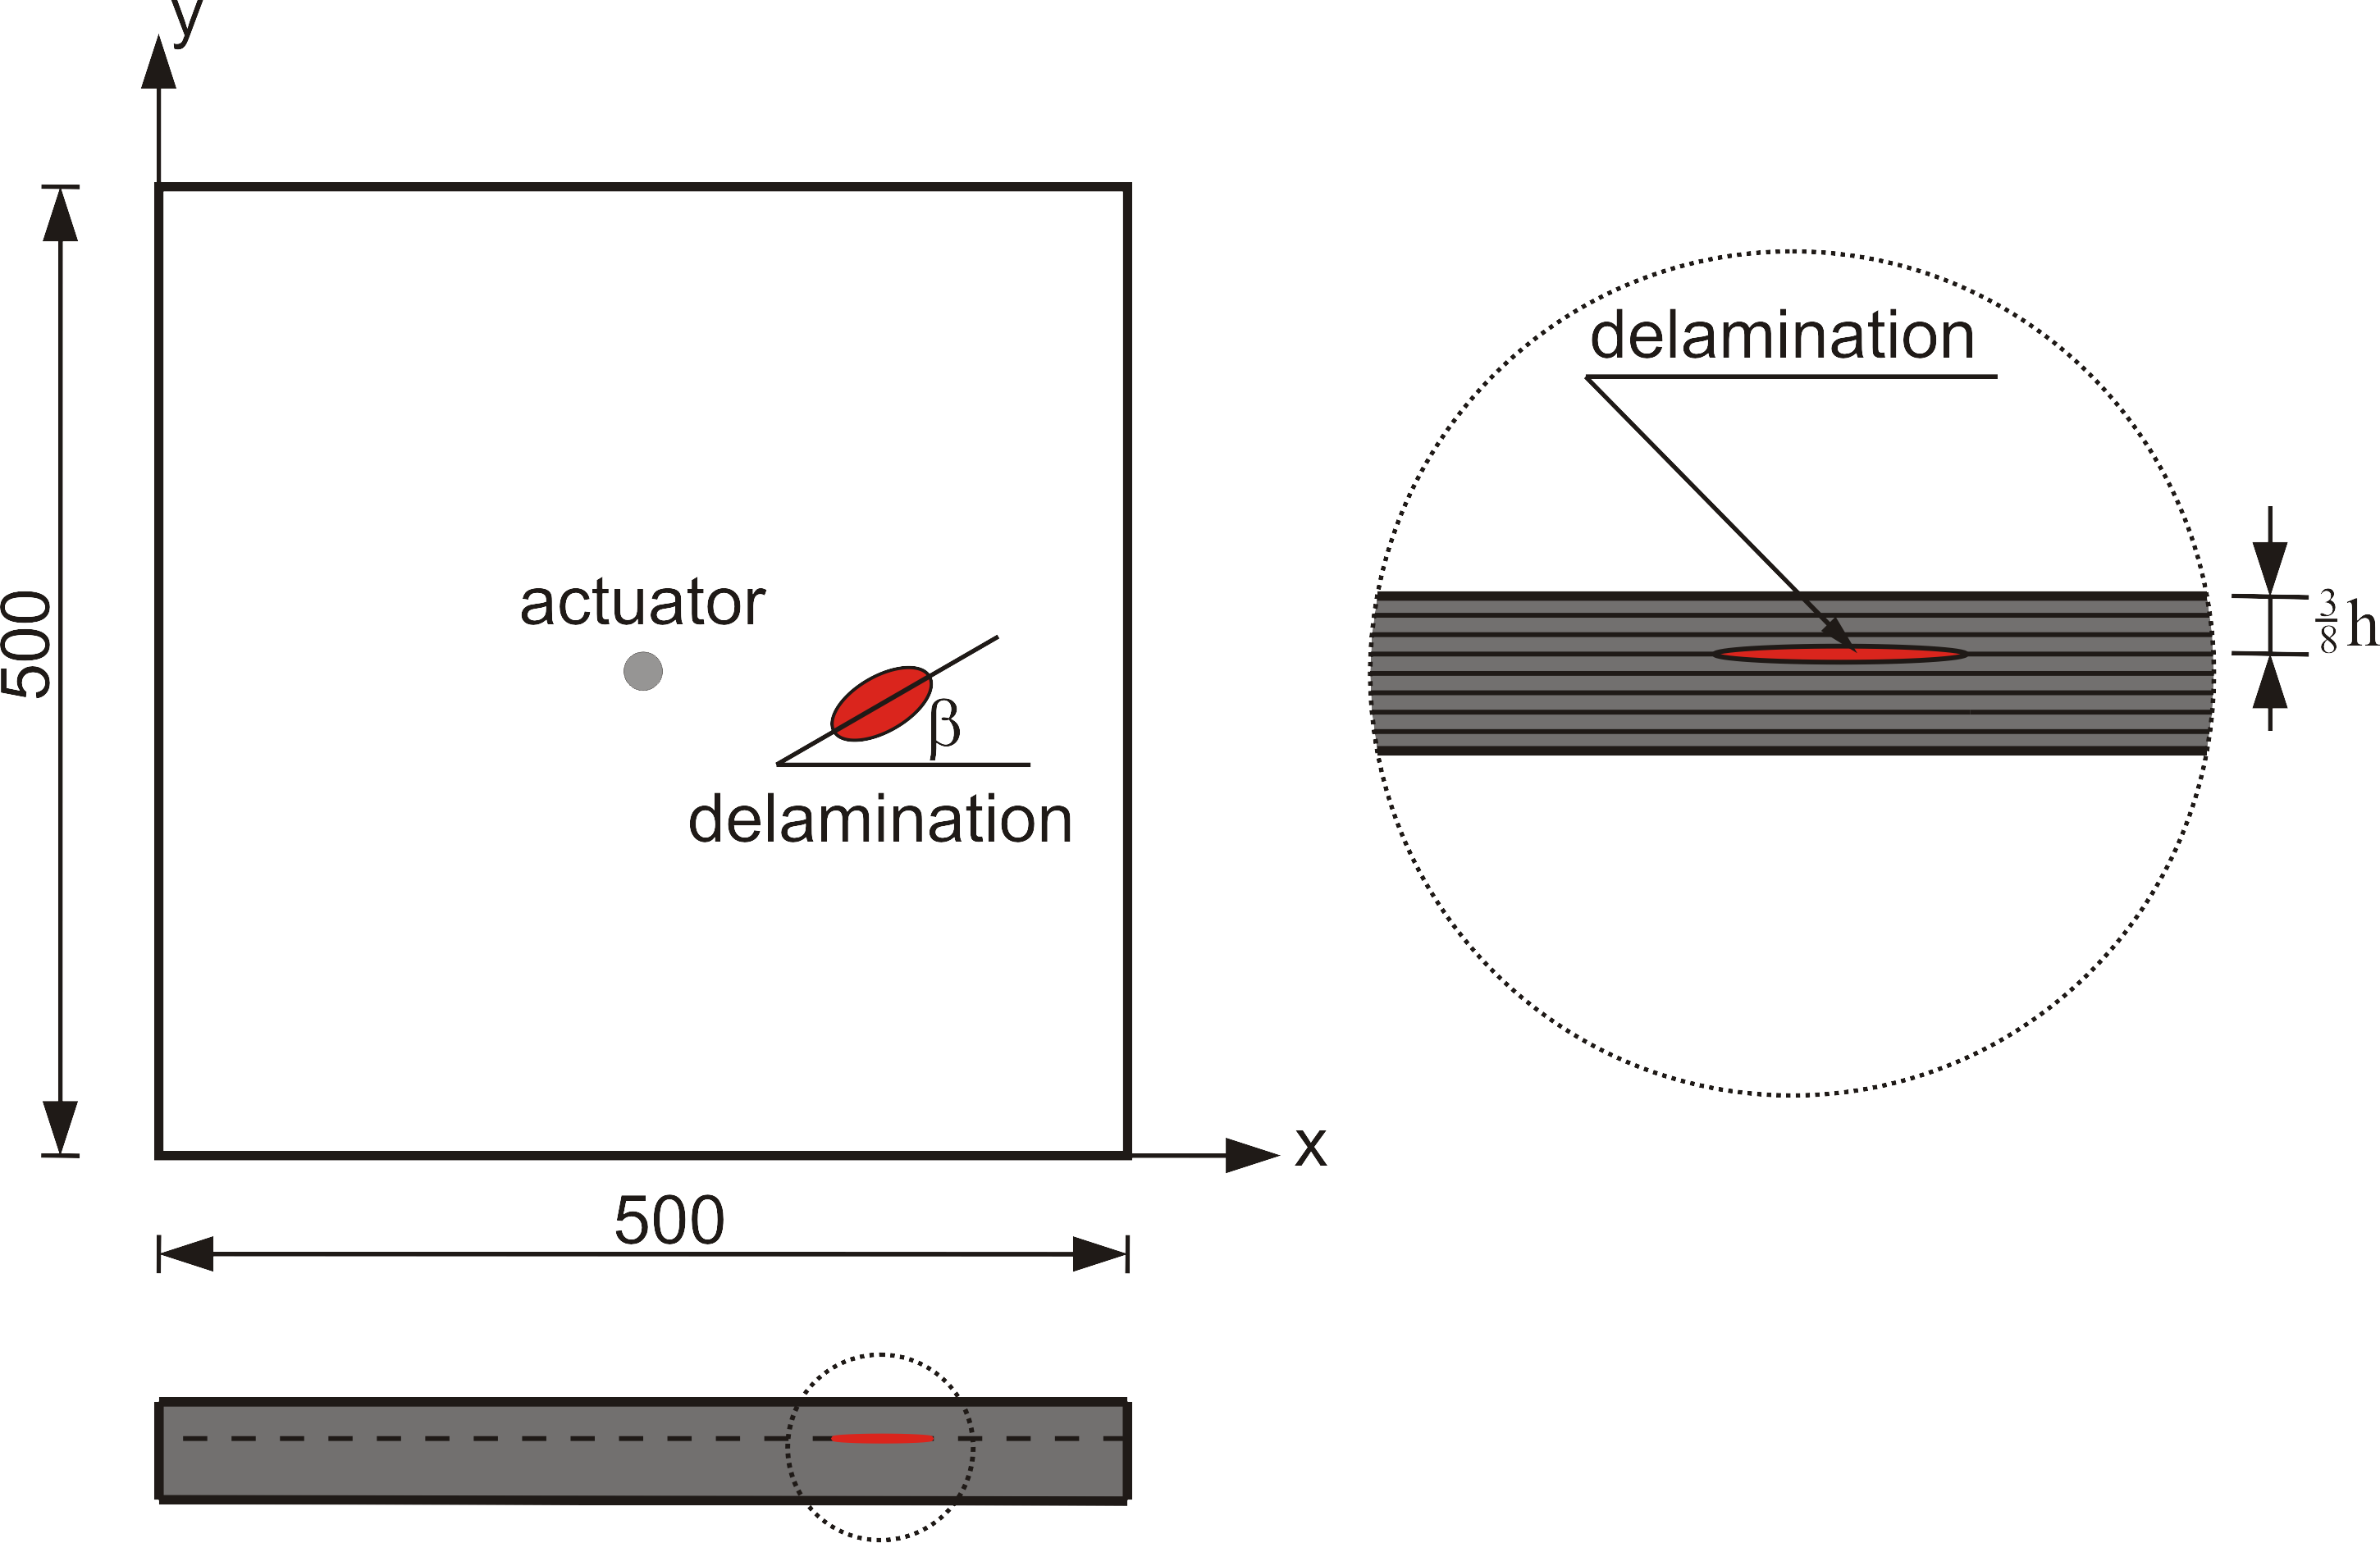
\includegraphics[scale=0.8]{plate_delam_arrangement_MSSP.png}
	\caption{Setup for computing Lamb wave interactions with delamination.}
	\label{fig:plate_setup}
\end{figure}	
	
Guided waves were excited at the plate centre by applying equivalent piezoelectric forces.
The excitation signal had a form of sinusoid modulated by Hann window. 
It was assumed that the carrier frequency is 50 kHz and the modulation frequency is 10 kHz.

The output from the top and bottom surfaces of the plate in the form of particle velocities at the nodes of spectral elements were interpolated on the uniform grid of 500\(\times\)500 points by using shape functions of elements (see~\cite{Kudela2020} for more details).
It essentially resembles measurements acquired by SLDV in the transverse direction (perpendicular to the plate surface).
An example of the simulated full wavefield data on the top and bottom surfaces is presented in Fig.~\ref{fig:wavefield}.
It should be noted that stronger wave entrapment at delamination can be observed for the case of the wavefield at the top surface.
It is because the delamination within cross-section is located closer to the top surface.
It makes it easier to detect delamination by processing wavefield at the top surface.
It is better visible if the root mean square (RMS) according to Eq.~(\ref{eq:rms}) is applied to the wavefield.
The result of this operation is presented in Fig.~\ref{fig:rms}.
Based on the image analysis, the shape of the delamination can be easier to discern for the top case.
However, the methodology presented in this paper was applied to the more difficult case i.e. wavefield registered at the bottom surface of the plate.

\begin{figure} [h!]
	\centering
	\begin{subfigure}[b]{0.32\textwidth}
		\centering
		\includegraphics[scale=1]{96_flat_shell_Vz_1_500x500top.png}
		\caption{\(t=0.141\) ms}
		\label{fig:frame96top}
	\end{subfigure}
	\hfill
	\begin{subfigure}[b]{0.32\textwidth}
		\centering
		\includegraphics[scale=1]{128_flat_shell_Vz_1_500x500top.png}
		\caption{\(t=0.188\) ms}
		\label{fig:frame128top}
	\end{subfigure}
	\hfill
	\begin{subfigure}[b]{0.32\textwidth}
		\centering
		\includegraphics[scale=1]{164_flat_shell_Vz_1_500x500top.png}
		\caption{\(t=0.240\) ms}
		\label{fig:frame164top}
	\end{subfigure}	
	\hfill
	\begin{subfigure}[b]{0.32\textwidth}
		\centering
		\includegraphics[scale=1]{96_flat_shell_Vz_1_500x500bottom.png}
		\caption{\(t=0.141\) ms}
		\label{fig:frame96bottom}
	\end{subfigure}
	\hfill
	\begin{subfigure}[b]{0.32\textwidth}
		\centering
		\includegraphics[scale=1]{128_flat_shell_Vz_1_500x500bottom.png}
		\caption{\(t=0.188\) ms}
		\label{fig:frame128bottom}
	\end{subfigure}
	\hfill
	\begin{subfigure}[b]{0.32\textwidth}
		\centering
		\includegraphics[scale=1]{164_flat_shell_Vz_1_500x500bottom.png}
		\caption{\(t=0.240\) ms}
		\label{fig:frame164bottom}
	\end{subfigure}

	\caption{Full wavefield at the top surface (a)--(c) and the bottom surface (d)--(f), respectively, at selected time instances showing the interaction of guided waves with delamination.}
	\label{fig:wavefield}
\end{figure} 

\begin{figure} [h!]
	\centering
	\begin{subfigure}[b]{0.47\textwidth}
		\centering
		\includegraphics[scale=1]{RMS_flat_shell_Vz_1_500x500top.png}
		\caption{top}
		\label{fig:rmstop}
	\end{subfigure}
	\hfill
	\begin{subfigure}[b]{0.47\textwidth}
		\centering
		\includegraphics[scale=1]{RMS_flat_shell_Vz_1_500x500bottom.png}
		\caption{bottom}
		\label{fig:rmsbottom}
	\end{subfigure}
	\caption{RMS of the full wavefield from the top surface of the plate (a) and the bottom surface of the plate (b).}
\label{fig:rms}
\end{figure} 
%%%%%%%%%%%%%%%%%%%%%%%%%%%%%%%%%%%%%%%%%%%%%%%%%%%%%
%%%%%%%%%%%%%%%%%%%%%%%%%%%%%%%%%%%%%%%%%%%%%%%%%%%%%
%%%%%%%%%%%%%%%%%%%%%%%%%%%%%%%%%%%%%%%%%%%%%%%%%%%%%
\subsection{Signal processing strategy}
%%%%%%%%%%%%%%%%%%%%%%%%%%%%%%%%%%%%%%%%%%%%%%%%%%%%
Two signal processing strategies are applied: newly proposed image processing based on the FCN and conventional one which is the adaptive wavenumber filtering.
The former one is represented by the left branch on the scheme shown in~Fig.~\ref{fig:sig_proc_strategy} whereas the latter one is represented by the right branch.
The starting point for both approaches is the dataset consisted of frames of propagating guided waves.
However, the FCN takes as an input the RMS which combines all frames into one image. 
It essentially represents the spatial energy distribution of propagating waves.
In the adaptive wavenumber filtering method, all frames are utilised (right branch of Fig.~\ref{fig:sig_proc_strategy}).
The RMS is applied later on to output final damage map in the form of an image.

It should be noted that we tested two types of activation functions as a last layer of the FCN: softmax and sigmoid.
The former one gives the binary output which segments pixels in two categories: damaged and undamaged.
On the other hand, the threshold needs to be applied when the sigmoid activation function is used.
Also, damage maps resulted from the adaptive wavenumber filtering must be thresholded so that the area and shape of delamination can be estimated.

Finally, IoU is applied as a measure of delamination size, shape and location so that all presented approaches can be compared quantitatively. 
	\begin{figure}
		\centering
		\includegraphics[scale=0.8]{FCN_adaptive_filtering_diagram_MSSP.png}
		\caption{Diagram of signal processing strategy by the proposed Fully Convolutional Network (left branch) in comparison to signal processing utilising adaptive wavenumber filtering method (right branch). }
		\label{fig:sig_proc_strategy}
	\end{figure}
The particular blocks presented in the Fig.~\ref{fig:sig_proc_strategy} will be explained in more details in the next sections.
%%%%%%%%%%%%%%%%%%%%%%%%%%%%%%%%%%%%%%%%%%%%%%%%%%%%%
%%%%%%%%%%%%%%%%%%%%%%%%%%%%%%%%%%%%%%%%%%%%%%%%%%%%%
%
%%%%%%%%%%%%%%%%%%%%%%%%%%%%%%%%%%%%%%%%%%%%%%%%%%%%	
\subsection{Adaptive wavenumber filtering}
%%%%%%%%%%%%%%%%%%%%%%%%%%%%%%%%%%%%%%%%%%%%%%%%%%%%
Adaptive wavenumber filtering is a well-established method for processing of images of propagating elastic waves.
The method has proved to be useful for crack size estimation~\cite{Kudela2015}, impact induced damage assessment~\cite{Kudela2018},  delamination and disbonding detection and localisation~\cite{Radzienski2019}.  
It is used here as a reference point for comparison purposes against proposed strategies based on FCN.

The method involves steps such as 2D Fourier Transform, wavenumber filtering, inverse Fourier Transform and RMS.
It can be used as an automated tool for producing damage maps which are easy in interpretation.
However, it still requires setting a threshold for the filter mask and quantisation threshold useful for damage size estimation.
These thresholds can be estimated empirically and even certain rigid range of thresholds will lead to satisfactory results.
Nevertheless, it is not a fully automatic process.
FCN based approach seems to have an advantage in this regard.
%%%%%%%%%%%%%%%%%%%%%%%%%%%%%%%%%%%%%%%%%%%%%%%%%%%%%
%%%%%%%%%%%%%%%%%%%%%%%%%%%%%%%%%%%%%%%%%%%%%%%%%%%%%
%%%%%%%%%%%%%%%%%%%%%%%%%%%%%%%%%%%%%%%%%%%%%%%%%%%%%
%\subsection{Fully Convolutional Network approach}
%%%%%%%%%%%%%%%%%%%%%%%%%%%%%%%%%%%%%%%%%%%%%%%%%%%%%%
%In this section, a deep learning approach for delamination detection in composite materials is presented. 
%%%%%%%%%%%%%%%%%%%%%%%%%%%%%%%%%%%%%%%%%%%%%%%%%%%%%
\subsection{Data preprocessing}
%%%%%%%%%%%%%%%%%%%%%%%%%%%%%%%%%%%%%%%%%%%%%%%%%%%%%
The wave propagation model produces outputs in the form of a 3D matrix which contains the propagating waves' amplitudes at location \((x, y)\) and time \(t\). 
Therefore, it can be seen as a set of frames of waves which propagates at a discrete-time moments \(t_k\).

Furthermore, the data preprocessing include a step of computation of root mean square (RMS) value as shown in Eqn.~\ref{eq:rms}, where \(N=512\) represents the sampling points.
\begin{equation}
	\hat{s}(x,y) = \sqrt{\frac{1}{N}\sum_{k=1}^{N} s(x,y,t_k)^2}
	\label{eq:rms}
\end{equation}
As a result, a 475 2D matrices were generated in which the amplitudes were stored as double-precision values.
Next, we have converted these matrices into grayscale images (colour image quantization).

To enhance the performance of the optimizer during the training process, the colour scale values were normalized to a range of (\(0-1\)) instead of the initial scale which was in a range of (\(0 - 255\)).	
Furthermore, we have applied data augmentation on the dataset by flipping the images horizontally, vertically and diagonally. 
As a result, the dataset size increased four times -- \(1900\)  images were produced.
By doing so, we can enhance the learning process by enabling the model to learn and recognise new and different complex patterns.
We have split the dataset into two portions:  \(80\%\) for the training set and \(20\%\) for the testing set.
Moreover, a cross-validation (CV) method was applied to the training set to reduce the overfitting issue. 
Fig.~\ref{fig:Cross_validation} illustrates as the CV method in which  we have applied a technique called k-fold CV.
In this technique, we have split the training set into \(k\) small sets (folds), hence the name k-folds. 
Therefore, we iterate over the training set k rounds.
During each round, the model uses  \(k-1\) folds for training and the remaining fold is used for validation. 
In our models, we choose \(k=5\), therefore, we have \(5\) rounds of training. 
%%%%%%%%%%%%%%%%%%%%%%%%%%%%%%%%%%%%%
For each round, we compute the performance of the model.
Finally, we compute the cross-validation performance for all rounds as illustrated in eqn.~\ref{eq:cv_performance} as a mean value over the k performance estimations of the validation fold set.
The main advantage of the K-fold CV method versus a regular train/test split is to reduce the overfitting by utilising data more efficiently as every data sample is used in both training and validation. 
Therefore, using by using this method we aim to improve the model ability to generalise and reduce the overfitting.
%%%%%%%%%%%%%%%%%%%%%%%%%%%%%%%%%%%%%
\begin{equation}
Final \ Performance = \frac{1}{k}\sum_{i=1}^{k}Performace
\label{eq:cv_performance}
\end{equation}
\begin{figure}
	\centering
	\includegraphics[scale=1.0]{cross_validation.png}
	\caption{K-fold Cross validation,\(k=5\).}
	\label{fig:Cross_validation}
\end{figure}
%%%%%%%%%%%%%%%%%%%%%%%%%%%%%%%%%%%%%%%%%%%%%%%%%%%%%

%%%%%%%%%%%%%%%%%%%%%%%%%%%%%%%%%%%%%%%%%%%%%%%%%%%%%
%%%%%%%%%%%%%%%%%%%%%%%%%%%%%%%%%%%%%%%%%%%%%%%%%%%%%
%%%%%%%%%%%%%%%%%%%%%%%%%%%%%%%%%%%%%%%%%%%%%%%%%%%%%
\subsubsection{The basic concept of Fully Convolutional Network}
%%%%%%%%%%%%%%%%%%%%%%%%%%%%%%%%%%%%%%%%%%%%%%%%%%%%%
The main purpose of such approach is to automatically perform feature extraction by training a model using full wavefield images, hence, it will learn by itself to recognise the patterns and detect the delamination and localize it.
In our work we are using the fully convolutional network (FCN)~\cite{long2015fully}, which aims to perform pixel-wise segmentation by classifying every pixel of the input image as damaged or not. 

The idea behind FCN is to stack a group of convolutional layers in an encoder-decoder style. 
The encoder is capable for downsampling the input image through convolutions with strides, consequently, resulting in a compressed feature representation of the input image, and the decoder is capable to upsample the image with compressed features applying techniques like transposed convolution with strides and upsampling with interpolation (e.g. bilinear or nearest).


In order to reduce overfitting in the models, some techniques were applied such as adding dropouts to layers.

For the output layer, we have applied two activation functions in separate experiments, the first one is softmax and the second one is sigmoid. 
The softmax function calculates the probability of the damage occurrence and the healthy state for every single pixel, hence, the summation of the two probabilities must equal one. Eq.~\ref{softmax} illustrates the softmax, where \(P(x)_{i}\) is the probability of each target class \(x_{j}\) over all possible target classes \(x_{j}\), C in our case are two classes  (damaged and undamaged).
To predict the output label of the detection (\(y_{pred}\)) which represent the probability of damaged and undamaged, we applied the \(\argmax\) function to select the maximum probability of the softmax activation function.
	\begin{equation}
		P(x)_{i} = \frac{e^{x_{i}}}{\sum_{j}^{C} e^{x_{j}}}
		\label{softmax}
	\end{equation} 
	\begin{equation}
		y_{pred} = \argmax_{i}\left( P(x)_{i} \right)
		\label{argmax}
	\end{equation}

When using sigmoid which in the output layer, it produces a vector of values between (\(0\) and \(1\)) indicating the damage weight for each pixel. 
Low values indicate low damage probability and high output values indicate high damage probability. Eq.~\ref{sigmoid} illustrates the sigmoid function, where \(z\) is the summation of adjustable weights \(\{w_0,w_1,...,w_n \}\) multiplied by input variables (from previous layer) \(\{x_0,x_1,_...,x_n\}\) and a bias \(b\) as shown in Eq~\ref{z}.	
	\begin{equation}
		\sigma(z) = \frac{1}{1+e^{-z}}
		\label{sigmoid}
	\end{equation}
	\begin{equation}
		z= \sum_{i=0}^{n}  w_i\, x_i +b
		\label{z}
	\end{equation}
Selecting the loss function is a crucial task in deep learning since it measures how good the model predicts.
We have applied two types of losses based on the used function in the final activation layer: binary cross-entropy (BCE) loss function applied with a sigmoid activation function in the output layer, categorical cross-entropy (CCE) loss function with a softmax activation in the output layer which is also called softmax loss function.
Eq.~\ref{BCE} illustrates the BCE, where \(\hat{Y}\) represents the predicted vector values and \(Y\) represents the ground truth vector values, when \(\hat{Y} \approx Y\) then the BCE will be almost \(0\) meaning that the model was able to predict the output, so, the aim is to reduce the loss function to the minimum value.
	\begin{equation}
		BCE = (1-Y)\log(1-\hat{Y})+Y\log(\hat{Y})
		\label{BCE}
	\end{equation}
Eq.~\ref{CCE} illustrates the CCE, where \( P(x)_{i}\) is the softmax value of the target class. 
	\begin{equation}
	CCE = -\log\left( P(x)_{i} \right)
	\label{CCE}
	\end{equation}

Moreover, we have applied intersection over union (IoU) as our accuracy metric. 
IoU is applied to find the intersection area between the ground truth value and the predicted value.  
The IoU metric is defined as:
\begin{equation}
IoU = \frac{Intersection}{Union} = \frac{\hat{Y} \cap Y}{\hat{Y} \cup Y} 
\label{IoU}
\end{equation}
The intersection between the predicted and the ground truth values is simply calculated through multiplying their values then summing the resulted values.
As we mentioned earlier the ground truth values are either \((0\) or \(1)\) thus only the predicted values larger than \(0\) multiplied by their ground truth label \(1\) will be counted, the rest values will equal to \(0\). 
The union can be calculated by summing all values in both the predicted and the ground truth  vectors, then we subtract the intersection from their sum.
Our main goal is to maximize the IoU accuracy metric, since the higher the IoU, the higher the accuracy of the predicted delamination in terms of location, shape and size.
	
Furthermore, during training the model our focus is to minimize the loss and maximize the accuracy metric by converting it into an optimization problem. 
The optimizer is responsible for updating the model learnable parameters such as filters weights and biases in a way the overall loss is minimized and the accuracy is maximized.
In the proposed approach, Adam optimizer was applied, which is considered as a combination of RMSprop and Stochastic Gradient Descent (SGD)~\cite{Kingma2015}. 

In the next subsection we are going to present a FCN model for pixel wise semantic segmentation in order to detect and localize delaminations.

%%%%%%%%%%%%%%%%%%%%%%%%%%%%%%%%%%%%%%%%%%%%%%%%%%%%%
%%%%%%%%%%%%%%%%%%%%%%%%%%%%%%%%%%%%%%%%%%%%%%%%%%%%%
\subsubsection{Residual UNet model}
%%%%%%%%%%%%%%%%%%%%%%%%%%%%%%%%%%%%%%%%%%%%%%%%%%%%%%%%%%%%%%%%%%%%%%%%%%%%%%%%
Residual UNet (Res-UNet) model is based on the residual learning~\cite{He2016} and the UNet technique~\cite{Ronneberger2015}. 
It is a well-known architecture that performs a biomedical segmentation based on encoder-decoder. 
The Res-UNet has a U-shape convolutional network that is based on encoder-decoder style. 
The encoder (contracting) path is responsible for capturing the detailed context of an input image, while the decoder (expansive) path is responsible for enabling a precise localisation. 
Hence, to maintain the spatial and contextual information from the previous layers from being lost residual connections were added at two levels:
\begin{itemize}
	\item at each step of the encoder and decoder paths,
	\item between the encoder parts and their corresponding decoder parts (skip connections) which ensures that the feature maps which were learned during the downsampling will be utilized in the reconstruction. 
\end{itemize}
The applied Res-UNet architecture is presented in Fig.~\ref{fig:Unet}.
%%%%%%%%%%%%%%%%%%%%%%%%%%%%%%%%%%%%%%%%%%%%%%%%%%%%%%%%%%%%%%%%%%%%%%%%%%%%%%%%
The encoder part holds several downsampling (Max-pool) blocks. 
Each block applies two convolutional layers followed by a (\(2\times2\)) max pooling with a (\(2\times2\)) strides that picks the maximum value in a local pool filter in one feature map (or \(n\)-feature maps), resulting in a reduction in the dimension of feature maps~\cite{Lecun2015}, consequently, reducing computation complexity.
Each convolutional layer performs (\(3\times3\)) convolution operations, followed by batch normalization (BN) then a Relu is applied.
Moreover, the number of convolutional filters is doubled after each downsampling block therefore the model can learn complex patterns effectively. 
%%%%%%%%%%%%%%%%%%%%%%%%%%%%%%%%%%%%%%%%%%%%%%%%%%%%%%%%%%%%%%%%%%%%%%%%%%%%%%%%
The bottleneck layer lies in between the encoder and the decoder as a joining point in the deepest layer in the model.
The bottleneck contains two convolutional layers, with \(1024\) filters which helps the model to learn and recognize the complex patterns.
%%%%%%%%%%%%%%%%%%%%%%%%%%%%%%%%%%%%%%%%%%%%%%%%%%%%%%%%%%%%%%%%%%%%%%%%%%%%%%%%
The decoder consists of several upsampling blocks. 
Each upsampling block passes the input into two convolution layers as in the downsampling block followed by a transmission up layer consisting of a transposed convolutional layer (upsampling). 
The purpose of upsampling is to retrieve the dimensions and increase the resolution.
Transposed convolutional layer differs from the regular upsampling function, by introducing learnable parameters regarding the transposed convolution filters that enhance the learning process of the model. 
Moreover, after each upsampling operation, the number of feature maps used by convolutional layer is reduced by half to keep the model symmetrical. 
%%%%%%%%%%%%%%%%%%%%%%%%%%%%%%%%%%%%%%%%%%%%%%%%%%%%%%%%%%%%%%%%%%%%%%%%%%%%%%%%
\begin{figure} [h!]
	\begin{center}
		\includegraphics[scale=1.0]{RES_UNET.png}
	\end{center}
	\caption{Res-UNet architecture.} 
	\label{fig:Unet}
\end{figure}
%%%%%%%%%%%%%%%%%%%%%%%%%%%%%%%%%%%%%%%%%%%%%%%%%%%%%%%%%%%%%%%%%%%%%%%%%%%%%%%%
\subsubsection{VGG16 encoder-decoder}
%%%%%%%%%%%%%%%%%%%%%%%%%%%%%%%%%%%%%%%%%%%%%%%%%%%%%%%%%%%%%%%%%%%%%%%%%%%%%%%%
In this model, we address the use of VGG16~\cite{Simonyan2015} architecture as a backbone encoder to the UNet~\cite{Ronneberger2015} technique.
VGG16 is composed of 13 convolutional layers, pooling layers and \(3\) dense layers, and it is used for classification purposes.
We removed the dense layers from the model, and we applied VGG16 of 13 convolutional layers as encoder-decoder for pixel-wise image segmentation.
Figure~\ref{vgg16} presents the architecture of VGG16 encoder-decoder model. 
The model has a U-shape of two parts: encoder and decoder.
The encoder consists of \(5\) convolutional blocks with a total \(13\)  (\(3\times3\)) convolutional layers followed by BN and activation function Relu.
A Max pool operation with pool size of (\(2\times2\)) followed by dropout is performed after each convolutional block.  
The upsampling path is introduced to recover spatial resolution, it also has \(5\) convolutional blocks with a total \(13\) \((3\times 3)\) convolutional layers.
For upsampling, bilinear interpolation with (\(2\times2\)) kernel size is applied.
Skip connections were added between downsampling blocks and the corresponding upsampling blocks in order to enhance recovering fine-grained details by enabling feature re-usability from earlier layers.
\begin{figure} [h!]
	\begin{center}
		\includegraphics[scale=1.0]{VGG16_encoder_decoder.png}
	\end{center}
	\caption{VGG16 encoder decoder architecture.} 
	\label{vgg16}
\end{figure}
%%%%%%%%%%%%%%%%%%%%%%%%%%%%%%%%%%%%%%%%%%%%%%%%%%%%
\subsubsection{FCN-DenseNet model}
%%%%%%%%%%%%%%%%%%%%%%%%%%%%%%%%%%%%%%%%%%%%%%%%%%%%%	
The one hundred layer tiramisu model (FCN-DenseNet) was introduced by Simon Jegou et al.~\cite{Jegou} for semantic segmentation.
FCN-DenseNet is similar to the U-Net architecture, FCN-DenseNet utilises the U-shape of the encoder-decoder scheme with skip connections between the downsampling and the upsampling paths to increase the resolution to the final feature map.
%Skip connections from the downsampling path to the corresponding upsampling path are essential for recovering spatially detailed information by reusing feature maps.

The main component in FCN-DenseNet is the dense block.
The purpose of the dense block is to concatenate layer input (feature maps) with its output (feature maps) to emphasize spatial details information.
The dense block is constructed from \(n\) varying number of layers, each layer is composed of a series of operations.
Figure~\ref{dense_block} illustrates the architecture of the dense block.
\begin{figure} [h!]
	\begin{center}
		\includegraphics[scale=1.0,angle=-90]{DenseBlock_layer.png}
	\end{center}
	\caption{Dense block architecture.} 
	\label{dense_block}
\end{figure}
%It has an input (\(x\)) (input image or output of transition layer) with \(k\) feature maps which is concatenated with the output of first layer and this process is recursively performed for all layers in the dense block ending up with output (\(y\)) with a (\(n\times k\)) feature maps. 
%%%%%%%%%%%%%%%%%%%%%%%%%%%%%%%%%%%%%%%%%%%%%%%%%%%%%%%%%%%%%%%%%%%%%%%%%%%%%%%%%%%%%%%%
Transition down layer was introduced to reduce the spatial dimensionality of the feature maps by performing a (\(1\times 1\)) convolution followed by (\(2\times2\)) Maxpool operation. 
%%%%%%%%%%%%%%%%%%%%%%%%%%%%%%%%%%%%%%%%%%%%%%%%%%%%%%%%%%%%%%%%%%%%%%%%%%%%%%%%%%%%%%%%
For the transition up layer, it was introduced in FCN-DenseNet to recover the input spatial resolution, to do that a transpose convolution operation is performed which upsamples the previous feature maps.
%%%%%%%%%%%%%%%%%%%%%%%%%%%%%%%%%%%%%%%%%%%%%%%%%%%%%%%%%%%%%%%%%%%%%%%%%%%%%%%%%%%%%%%%
Feature maps emerging from upsampling are concatenated with the ones resulting from the skip connection forming the input to a new dense block.
During the upsampling, the input to the dense block is not concatenated with its output to overcome the overhead of memory shortage since the upsampling path expands the spatial resolution of the feature maps.
Table~\ref{layers} presents the architecture of a single layer, the transition down  and transition up layers in details.
Figure~\ref{fcn} illustrates the FCN-DenseNet architecture for image segmentation used for delamination detection.
%%%%%%%%%%%%%%%%%%%%%%%%%%%%%%%%%%%%%%%%%%%%%%%%%%%%%%%%%%%%%%%%%%%%
\begin{table}[h!]
	\renewcommand{\arraystretch}{1.3}
	\centering
	\scriptsize
	\begin{tabular}{|c|l|c|l|c|}
		\cline{1-1} \cline{3-3} \cline{5-5}
		\textbf{Layer} &  & \textbf{Transition Down} &  & \textbf{Transition Up} \\ \cline{1-1} \cline{3-3} \cline{5-5} 
		Batch Normalization &  & Batch Normalization &  & \multirow{5}{*}{\begin{tabular}[c]{@{}c@{}}(\(3\times3\)) Transposed Convolution, \\ strides = (\(2\times2\))\end{tabular}} \\ \cline{1-1} \cline{3-3}
		Relu &  & Relu &  &  \\ \cline{1-1} \cline{3-3}
		(\(3\times3\)) Convolution &  & (\(1\times1\)) Convolution &  &  \\ \cline{1-1} \cline{3-3}
		\multirow{2}{*}{Dropout \(p = 0.2\)} &  & Dropout \(p = 0.2\) &  &  \\ \cline{3-3}
		&  & (\(2\times2\)) Maxpooling &  &  \\ \cline{1-1} \cline{3-3} \cline{5-5} 
	\end{tabular}
	\caption{Layer, Transition Down and Transition Up layers.} 
	\label{layers}
\end{table}\\

\begin{figure} [h!]
	\begin{center}
		\includegraphics[scale= 1.0]{FCN_dense_net.png}
	\end{center}
	\caption{FCN-DenseNet architecture.} 
	\label{fcn}
\end{figure}
%Our constructed model is composed of \(3\) dense blocks in the downsampling path, one dense block in bottleneck and 3 dense blocks for the upsampling path. 
%Each dense block in the downsampling and upsampling paths consists of \(2\) layers, the bottleneck dense block consists of \(4\) layers.
%The model input is the RMS image with size of (\(512\times 512\)).
%At the beginning, we perform a  convolution operation and concatenate the original input with the output, then the concatenated output is fed into the first dense block that consists of (\(2\)) layers.
%
%Each layer is composed of Ronneberger2015normalization (BN) followed by Relu, then (\(3\times3\)) convolution with same padding is applied followed by a dropout with probability \(p = 0.2\).
%Then, the output of the first dense layer is concatenated with its input and is fed into a transition down layer. 
%
%The transition down layer is composed of BN followed by Relu, then (\(1\times1\)) convolution followed by a dropout with probability \(p = 0.2\) and finally (\(2\times2\)) Maxpool with strides of (\(2\times2\)).
%
%This process is repeated until the bottleneck dense block.
%The bottleneck dense block consists of 4 layers.
%The output of the bottleneck is directed into the upsampling path starting with transition up layer.
%Accordingly, the output of the transition up layer is concatenated with the corresponding dense block output in the downsampling path.
%The final layer in the network is  (\(1\times1\)) convolution followed by either a sigmoid function or a softmax function to calculate the probability of damage for each pixel.
%Hence, we have two versions of the FCN-DenseNet model with different output layer function.

%%%%%%%%%%%%%%%%%%%%%%%%%%%%%%%%%%%%%%%%%%%%%%%%%%%%%
%%%%%%%%%%%%%%%%%%%%%%%%%%%%%%%%%%%%%%%%%%%%%%%%%%%%%
\subsubsection{Pyramid Scene Parsing Network}
	%%%%%%%%%%%%%%%%%%%%%%%%%%%%%%%%%%%%%%%%%%%%%%%%%%%%
	Pyramid Scene Parsing Network (PSPNet) proposed by Zhao et al.~\cite{zhao2017pyramid} is a state-of-the-art deep learning model for image segmentation. PSPNet is a multi-scale network that effectively learns the global context representation of a scene. PSPNet employes residual network (ResNet)~\cite{he2016deep}, with a dilated network as a feature extractor for the extraction of various patterns from the input image. ResNet designed by He et al.~\cite{he2016deep} is very popular due to its depth (up to 152 layers) and with the inclusion of residual blocks. The residual blocks are very useful for training a really deep neural network by proposing the skip connections in such a way that layers can mimic their inputs to the succeeding layer. 
	This approach assures that the subsequent layer has learned something new and different from what the input has already been encoded. Additionally, such connections help to overcome the vanishing gradients problem. These days, ResNet is commonly applied for feature extraction in various deep CNN models. 
	
	PSPNet renders an adequate global contextual information for pixel-level scene parsing. The local and global clues together provide a more reliable predictions. Sub-regions context along with global context information is very useful for distinguishing among different kinds of objects. For further reducing context information loss among diverse sub-regions, a hierarchical global prior was proposed. The hierarchical global prior contains information of multiple scales and it varies among different sub-regions. The pyramid pooling module combines features under four distinct pyramid scales, however, the number of these pyramid levels and size of each level can be modified because they are related to the size of the feature map that is fed into the pyramid pooling layer. The coarsest level highlighted as red in Fig. is employing global pooling for producing a single bin output. The feature map is separated into different sub-regions in the subsequent pyramid levels and form pooled representation for different locations.
	
	The distinctive levels of the pyramid pooling module generate an output of the feature map of different sizes. These feature maps are processed with a 1 x 1 convolutional layer to reduce their dimensions. The output of the pyramid levels is then up-sampled with bilinear interpolation before the concatenation with the initial feature maps to obtain both local and global context information. In the end, a convolutional layer is employed for generating the pixel-wise segmented predictions. 
	
\begin{comment}
	Our pyramid pooling module is a four-level one with bin
	sizes of 1 x 1, 2 x 2, 3 x 3 and 6 x 6 respectively.
	Given an input image in Fig. 3(a), we use a pretrained
	ResNet [13] model with the dilated network strategy [3, 40]
	to extract the feature map. The final feature map size is 1/8
	of the input image, as shown in Fig. 3(b). On top of the map, we use the pyramid pooling module shown in (c) to gather context information. Using our 4-level pyramid, the pooling kernels cover the whole, half of, and small portions of the image. They are fused as the global prior. Then we
	concatenate the prior with the original feature map in the
	final part of (c). It is followed by a convolution layer to generate the final prediction map in (d). 
	
	Figure 3. Overview of our proposed PSPNet. Given an input image (a), we first use CNN to get the feature map of the last convolutional
	layer (b), then a pyramid parsing module is applied to harvest different sub-region representations, followed by upsampling and concatenation
	layers to form the final feature representation, which carries both local and global context information in (c). Finally, the representation
	is fed into a convolution layer to get the final per-pixel prediction (d).
		
	Fig. 17. The PSPNet architecture. A CNN produces the feature map
	and a pyramid pooling module aggregates the different sub-region
	representations. Up-sampling and concatenation are used to form the
	final feature representation from which, the final pixel-wise prediction is
	obtained through convolution. From [57].
	
	Fig. 17. PSPNet architecture. Initial feature maps (b) are extracted from input images (a) by using a pretrained ResNet [18] alongside dilated network strategy. Pyramidpooling module (c) covers from the whole, half of to small regions of the image. Finally, initial feature map is concatenated with pooling module output and applying aconvolution layer final predicted maps (d) are generated.
	
	Fig. 10 Overview of the pyramid scene parsing networks. Given an input image (a), feature maps from last
	convolution layer are pulled (b), then a pyramid parsing module is applied to harvest different sub-region
	representations, followed by upsampling and concatenation layers to form the final feature representation,
	which carries both local and global context information in c. Finally, the representation is fed into a convolution
	layer to get the final per-pixel prediction (d) Zhao et al. (2017b)
\end{comment}
%%%%%%%%%%%%%%%%%%%%%%%%%%%%%%%%%%%%%%%%%%%%%%%%%%%%%
%%%%%%%%%%%%%%%%%%%%%%%%%%%%%%%%%%%%%%%%%%%%%%%%%%%%%
\section{Results and Discussions}
%%%%%%%%%%%%%%%%%%%%%%%%%%%%%%%%%%%%%%%%%%%%%%%%%%%%%
In this section, four deep learning models  of semantic segmentation approach including UNet, VGG16 encoder-decoder, FCN-DenseNet and PSPNet were evaluated on three damage scenarios  which were numerically generated in order to identify the delamination.
Additionally, an experimental scenario was also used to evaluate the performance of the models to show the deep learning capabilities of generalization.
For each model, the mean IoU is calculated and presented as a metric of comparison.

In our work, all semantic segmentation models were implemented and trained with Keras API~\cite{chollet2015keras} (an open-source platform) running on top of TensorFlow on a GeForce RTX 2080 GPU from NVIDIA. 
Moreover, for training purposes, we have used K-fold CV technique with \(k=5\), which means each model has trained for \(5\) iterations and finally the mean performance is calculated. 
Further, for each iteration, the models were trained on the augmented dataset up to \(100\) epochs.

The first delamination scenario is shown in Figure~\ref{fig:softmax_448}. 
The RMS of the full wavefield interpolated at the bottom surface of the plate with a delamination located the left edge of the plate and its corresponding ground truth image are shown in fig.~\ref{fig:RMS_flat_shell_Vz_448}, ~\ref{fig:m1_rand_single_delam_448} respectively. 
In fig.~\ref{fig:unet_pred_448} we presents the predicted output of the UNet model, the IoU = \(0.760\) for this case.
Figure~\ref{fig:vgg16_pred_448} show the predicted output of the VGG16 encoder-decoder model, and the IoU = \(0.841\). 
Figure~\ref{fig:pspnet_pred_448} shows the predicted output of PSPNet model, the IoU =\(0.747\).
The lase figure in the first scenario ~\ref{fig:fcn_densenet_pred_448}	show the predicted output of FCN-DenseNet model, the IoU=\(0.757\).
\begin{figure} [!h]
	\centering
	\begin{subfigure}[b]{0.47\textwidth}
		\centering
		\includegraphics[scale=1.0]{RMS_448.png}
		\caption{RMS bottom}
		\label{fig:RMS_flat_shell_Vz_448}
	\end{subfigure}
	\hfill
	\begin{subfigure}[b]{0.47\textwidth}
		\centering
		\includegraphics[scale=1.0]{GT_448.png}
		\caption{Ground truth}
		\label{fig:m1_rand_single_delam_448}
	\end{subfigure}
	\begin{subfigure}[b]{0.47\textwidth}
		\centering
		\includegraphics[scale=1.0]{unet_Pred_softmax_448.png}
		\caption{UNet}
		\label{fig:unet_pred_448}
	\end{subfigure}
	\hfill
	\begin{subfigure}[b]{0.47\textwidth}
		\centering
		\includegraphics[scale=1.0]{vgg16_encoder_decoder_Pred_softmax_448.png}
		\caption{VGG16 encoder-decoder}
		\label{fig:vgg16_pred_448}
	\end{subfigure}
	\hfill
	\begin{subfigure}[b]{0.47\textwidth}
		\centering
		\includegraphics[scale=1.0]{pspnet_Pred_softmax_448.png}
		\caption{PSPNet}
		\label{fig:pspnet_pred_448}
	\end{subfigure}
	\hfill
	\begin{subfigure}[b]{0.47\textwidth}
		\centering
		\includegraphics[scale=1.0]{fcn_densenet_Pred_softmax_448.png}
		\caption{FCN-DenseNet}
		\label{fig:fcn_densenet_pred_448}
	\end{subfigure}
	\caption{UNet, Vgg16 encoder-decoder, PSPNet, FC-DenseNet /  448}
	\label{fig:softmax_448}
\end{figure} 

The second delamination scenario is shown in Figure~\ref{fig:385_softmax}. 
The RMS of the full wavefield interpolated at the bottom surface of the plate with a delamination located the upper left corner of the plate and its corresponding ground truth image are shown in fig.~\ref{fig:RMS_flat_shell_Vz_385}, ~\ref{fig:m1_rand_single_delam_385} respectively. 

Numerical results for RMS\_385
UNet = \(0.691\), VGG16 encoder-decoder = \(0.770\), FCN-DenseNet =\(0.776\), PSPNet = \(0.867\)

	\begin{figure}[!h]
		\centering
		\begin{subfigure}[b]{0.47\textwidth}
			\centering
			\includegraphics[scale=1.0]{RMS_385.png}
			\caption{RMS bottom}
			\label{fig:RMS_flat_shell_Vz_385}
		\end{subfigure}
		\hfill
		\begin{subfigure}[b]{0.47\textwidth}
			\centering
			\includegraphics[scale=1.0]{GT_385.png}
			\caption{Ground truth}
			\label{fig:m1_rand_single_delam_385}
		\end{subfigure}
		\begin{subfigure}[b]{0.47\textwidth}
			\centering
			\includegraphics[scale=1.0]{unet_Pred_softmax_385.png}
			\caption{UNet}
			\label{fig:Unet_Pred__softmax_385}
		\end{subfigure}
		\hfill
		\begin{subfigure}[b]{0.47\textwidth}
			\centering
			\includegraphics[scale=1.0]{vgg16_encoder_decoder_Pred_softmax_385.png}
			\caption{VGG16 encoder-decoder softmax}			\label{fig:vgg16_pred__softmax_385}			
		\end{subfigure}
		\hfill
		\begin{subfigure}[b]{0.47\textwidth}
			\centering
			\includegraphics[scale=1.0]{pspnet_Pred_softmax_385.png}
			\caption{PSPNet}
			\label{fig:pspnet_pred__softmax_385}
		\end{subfigure}	
		\hfill
		\begin{subfigure}[b]{0.47\textwidth}
			\centering
			\includegraphics[scale=1.0]{fcn_densenet_Pred_softmax_385.png}
			\caption{FCN-DenseNet}
			\label{fig:fcn_densenet_pred__softmax_385}
		\end{subfigure}	
		\caption{UNet, Vgg16 encoder-decoder, PSPNet, FC-DenseNet / 385}
		\label{fig:385_softmax}
	\end{figure}
	%%%%%%%%%%%%%%%%%%%%%%%%%%%%%%%%%%%%%%%%%%%%%%%%%%%

The third delamination scenario is shown in Figure~\ref{fig:475_softmax}. 
The RMS of the full wavefield interpolated at the bottom surface of the plate with a delamination located the upper middle  of the plate and its corresponding ground truth image are shown in fig.~\ref{fig:RMS_flat_shell_Vz_475}, ~\ref{fig:m1_rand_single_delam_475} respectively. 

numerical results for RMS\_475
UNet = \(0.79\), VGG16 encoder-decoder = \(0.84\), FCN-DenseNet =\(0.38\), PSPNet = \(0.80\)
	
\begin{figure}[!h]
	\centering
	\begin{subfigure}[b]{0.47\textwidth}
		\centering
		\includegraphics[scale=1.0]{RMS_475.png}
		\caption{RMS bottom}
		\label{fig:RMS_flat_shell_Vz_475}
	\end{subfigure}
	\hfill
	\begin{subfigure}[b]{0.47\textwidth}
		\centering
		\includegraphics[scale=1.0]{GT_475.png}
		\caption{Ground truth}
		\label{fig:m1_rand_single_delam_475}
	\end{subfigure}
	\begin{subfigure}[b]{0.47\textwidth}
		\centering
		\includegraphics[scale=1.0]{unet_Pred_softmax_475.png}
		\caption{UNet softmax}
		\label{fig:Unet_Pred__softmax_475}
	\end{subfigure}
	\hfill
	\begin{subfigure}[b]{0.47\textwidth}
		\centering
		\includegraphics[scale=1.0]{vgg16_encoder_decoder_Pred_softmax_475.png}
		\caption{VGG16 encoder-decoder softmax}			\label{fig:vgg16_pred__softmax_475}			
	\end{subfigure}
	\hfill
	\begin{subfigure}[b]{0.47\textwidth}
		\centering
		\includegraphics[scale=1.0]{pspnet_Pred_softmax_475.png}
		\caption{PSPNet softmax}
		\label{fig:pspnet_pred__softmax_475}
	\end{subfigure}	
	\hfill
	\begin{subfigure}[b]{0.47\textwidth}
		\centering
		\includegraphics[scale=1.0]{fcn_densenet_Pred_softmax_475.png}
		\caption{FCN-DenseNet softmax}
		\label{fig:fcn_densenet_pred__softmax_475}
	\end{subfigure}	
	\caption{UNet, Vgg16 encoder-decoder, PSPNet, FC-DenseNet /  425}
	\label{fig:475_softmax}
\end{figure}
%%%%%%%%%%%%%%%%%%%%%%%%%%%%%%%%%%%%%%%%%%%%%%%%%%%
%	%%%%%%%%%%%%%%%%%%%%%%%%%%%%%%%%%%%%%%%%%%%%%%%%%%%
%	\begin{figure}[!h]
%		\centering
%		\begin{subfigure}[b]{0.47\textwidth}
%			\centering
%			\includegraphics[scale=1.0]{RMS_bottom_464.png}
%			\caption{RMS bottom}
%			\label{fig:RMS_flat_shell_Vz_464}
%		\end{subfigure}
%		\hfill
%		\begin{subfigure}[b]{0.47\textwidth}
%			\centering
%			\includegraphics[scale=1.0]{ground_truth_464.png}
%			\caption{Ground truth}
%			\label{fig:m1_rand_single_delam_464}
%		\end{subfigure}
%		\begin{subfigure}[b]{0.47\textwidth}
%			\centering
%			\includegraphics[scale=1.0]{Unet_Pred__softmax464.png}
%			\caption{UNet softmax}
%			\label{fig:Unet_Pred__softmax464}
%		\end{subfigure}
%		\hfill
%		\begin{subfigure}[b]{0.47\textwidth}
%			\centering
%			\includegraphics[scale=1.0]{vgg16_pred__softmax464.png}
%			\caption{VGG16 encoder-decoder softmax}			\label{fig:vgg16_pred__softmax464}			
%		\end{subfigure}
%		\hfill
%		\begin{subfigure}[b]{0.47\textwidth}
%			\centering
%			\includegraphics[scale=1.0]{pspnet_pred__softmax464.png}
%			\caption{PSPNet softmax}
%			\label{fig:pspnet_pred__softmax464}
%		\end{subfigure}	
%		\hfill
%		\begin{subfigure}[b]{0.47\textwidth}
%			\centering
%			\includegraphics[scale=1.0]{fcn_densenet_pred__softmax464.png}
%			\caption{FCN-DenseNet softmax}
%			\label{fig:fcn_densenet_pred__softmax464}
%		\end{subfigure}	
%		\caption{UNet, Vgg16 encoder-decoder, PSPNet, FC-DenseNet / softmax 464}
%		\label{fig:464_softmax}
%	\end{figure}
%	%%%%%%%%%%%%%%%%%%%%%%%%%%%%%%%%%%%%%%%%%%%%%%%%%%%
	
	
	
%In the next scenario, we present delamination located in the upper left part of the plate.
%Figs.~\ref{fig:dispersion30deg_direct}, ~\ref{fig:m1_rand_single_delam_454} show the RMS of the full wavefield interpolated at the bottom surface of the plate.
%Fig.~\ref{fig:ERMSF_flat_shell_Vz_454} shows the damage map obtained by using the adaptive wavenumber filtering.
%The adaptive wavenumber filtering method picks some noise at the edges but the shape of delamination is clearly highlighted by high values of damage map.
%Nevertheless, there is still some noise after applying threshold as it is shown in Fig.~\ref{fig:Binary_ERMSF}.
%The IoU for this case is \(0.61\).
%In Figs.~\ref{fig:predict_454_sigmoid_tr_0.5}, ~\ref{fig:predict_454_softmax} we present the FCN-DeneseNet outputs with sigmoid and softmax, respectively.
%The sigmoid detect the delamination with IoU = \(0.58\), and for the softmax with IoU = \(0.60\).
%As we can see also for this scenario, the FCN-DenseNet only detects the delamination patterns without unwanted noise.
	
%	Figs.[~\ref{fig:unthresholded438}, ~\ref{fig:unthresholded454}] show the original damage maps without thresholding for the FCN-DenseNet with sigmoid function for the first and second scenarios respectively. 
%	As shown from the figs, the predicted output has a range or probabilities of damage. 
%	Accordingly, we apply threshold to exclude these low damage probabilities.
%	\begin{figure} [!h] 
%		\centering
%		\begin{subfigure}[b]{0.47\textwidth}
%		\centering
%		\includegraphics[scale=1]{sigmoid_unthresholded438.png}
%		\caption{}
%		\label{fig:unthresholded438}
%		\end{subfigure}
%	\hfill	
%	\begin{subfigure}[b]{0.47\textwidth}
%		\centering 	
%		\includegraphics[scale=1]{sigmoid_unthresholded454.png}
%		\caption{}
%		\label{fig:unthresholded454}
%	\end{subfigure}
%	\caption{Unthresholded damage maps for FCN-DenseNet/sigmoid}
%	\label{fig:unthresholded}
%	\end{figure}

%In Fig.~\ref{fig:RMS433} we present the third scenario where the damage map obtained by the adaptive wavenumber filtering method is useful for delamination visualisation but the FCN-DenseNet model failed.
%%%%%%%%%%%%%%%%%%%%%%%%%%%%%%%%%%%%%%%%%%%%%%%%%%%
% third figure
%%%%%%%%%%%%%%%%%%%%%%%%%%%%%%%%%%%%%%%%%%%%%%%%%%%

%Figures.~\ref{fig:RMS_flat_shell_Vz_433}, ~\ref{fig:m1_rand_single_delam_433} show the RMS of the full wavefield interpolated at the bottom surface of the plate with delamination located at the upper left corner of the plate and its corresponding ground truth, respectively.
%It is impossible to notice any changes of RMS pattern caused by the delamination (Fig.~\ref{fig:RMS_flat_shell_Vz_433}).
%It should be noted that this image is fed to the FCN-DenseNet model whereas the full wavefield (all frames) are used in the adaptive wavenumber filtering method.
%In extreme cases, like this, conventional signal processing has an advantage over the FCN-DenseNet model.
%As shown in Fig.~\ref{fig:ERMSF_flat_shell_Vz_433} representing the damage map obtained by the adaptive wavenumber filtering technique, the delamination location can be identified by a well-trained expert. 
%However, the values of the damage map corresponding to the delamination location are on the same level as the noise.
%Hence, when binary thresholding is applied, only some false damage indications are highlighted near corners of the plate as show in Fig.~\ref{fig:Binary_ERMSF_flat_shell_Vz_433}. 
%For this case IoU= \(0\) for all considered methods.
% 
%Delaminations located near edges or corners are difficult to detect due to edge wave reflections which have similar patterns as delamination reflections. 
%The problem arises for both conventional and deep learning techniques. 
%However, to solve this issue for the FCN model, we need to enhance the feature extraction process by obtaining more data to train the model to recognise and learn new patterns.	
%
%In Table~\ref{tab:iou} we present the maximum, minimum and mean value of IoU for the adaptive filtering and FCN-DenseNet for sigmoid (threshold = \(0.5\)) and softmax for all testing images.
%	\begin{table}
%	 \renewcommand{\arraystretch}{1.3}
%		\centering
%		\caption{IoU for all models}
%		\label{tab:iou}
%		\resizebox{\textwidth}{!}{\begin{tabular}{ccccccccccccc}
%				\toprule
%				&  &  &  &  &  & \multicolumn{7}{c}{FCN-Dense Model} \\ \cline{7-13} 
%				&  & \multicolumn{3}{c}{Adaptive filtering} &  & \multicolumn{3}{c}{sigmoid} &  & \multicolumn{3}{c}{softmax} \\ \cline{3-5} \cline{7-9} \cline{11-13} 
%				&  & min & max & mean &  & min & max & mean &  & \multicolumn{1}{c}{min} & \multicolumn{1}{c}{max} & \multicolumn{1}{c}{mean} 
%				%\\ \cline{3-13} 
%				\\ \cline{3-5} \cline{7-9} \cline{11-13} 
%				\multicolumn{2}{c}{IoU} &0&0.648&0.373& &0&0.933&0.616&  &0&0.878&0.623\\ 
%				\bottomrule
%		\end{tabular}}
%	\end{table}
	
%Every single value of the IoU was estimated for all testing images using FCN-DenseNet with a sigmoid at the output layers.
%It is expected that as we increase the threshold, the IoU will decrease because some of the detected output values will be excluded.
%Therefore, selecting the proper threshold value is important for maximizing IoU. 
%Fig.~\ref{fig:iou_fcn} shows the maximum and mean IoU for all testing images depending on the threshold value. 
%The IoU is decreasing along with the threshold increment in the range of (\(0-1\)).
%
%Note that for each pixel we get a value between (\(0 to 1\)).
%We take 0.5 as the threshold to decide whether to classify a pixel as 0 or 1.
%However deciding threshold is tricky and can be treated as another hyper parameter.

%	\begin{figure}[!h] 
%		\centering
%		\includegraphics[width=\textwidth]{iou_all_models_sigmoid.png}
%		\centering
%		\caption{IoU for different models with sigmoid of a range of thresholds \((0.0-1.0)\)} 
%		\label{fig:iou_fcn}
%	\end{figure}
%	

\begin{table}[]
	\centering
	\caption{}
	\label{tab:table_iou}
	\begin{tabular}{ccc}
		\multicolumn{3}{c}{IoU} \\ \hline
		& mean & max \\ \hline
		U-Net & 0.67 & 0.93 \\ \hline
		VGG16 encoder-decoder & 0.66 & 0.90 \\ \hline
		FCN-DenseNet & 0.52 & 0.82 \\ \hline
		PSPNet & 0.66 & 0.93 \\ \hline
	\end{tabular}
	
\end{table}

\begin{table}[]
	\centering
	\caption{}
	\label{tab:table_parameters}
	\resizebox{\textwidth}{!}
	{
		\begin{tabular}{cccc}
			\multicolumn{4}{c}{Model parameters} \\ \hline
			& Trainable params & Non-trainable params & Total params \\ \hline
			U-Net & 2,161,378 & 2,944 & 2,164,322 \\ \hline
			VGG16 encoder-decoder & 5,287,282 & 5,760 & 5,293,042 \\ \hline
			FCN-DenseNet & 150,516 & 1,346 & 151,862 \\ \hline
			PSPNet & 912,370 & 3,744 & 916,114 \\ \hline
		\end{tabular}
	}

\end{table}

In Fig.~\ref{fig:Exp_ERMS_teflon}, we present an experimental scenario of CFRP with Teflon insert as artificial delamination.
Similarly to the numerical case, the frequency of \(50\) kHz was used to excite the transducer which was placed at the centre of the plate.
As shown in Fig.~\ref{fig:ERMSF_CFRP_teflon} the adaptive wavenumber filtering method is able to detect the delamination. 
Fig.~\ref{fig:Binary_ERMSF_CFRP} shows the binary thresholded output which precisely highlights the location of delamination. 
Even the shape of the delamination is quite well represented.
The IoU for this scenario was \(0.401\). 

%The FCN-DenseNet model detected the delamination with both a sigmoid and softmax functions as shown in Fig.~\ref{fig:EXP_predict_sigmoid} and Fig.~\ref{fig:EXP_predict_softmax}, respectively.
%The IoU for FCN-DenseNet model was \(0.053\) and \(0.081\) for a sigmoid and softmax, respectively.
%These poor results of predictions are expected since we trained our model only on numerically generated data.
%However, apart from the noise at the edges and at the transducer location, the FCN-DenseNet could detect the delamination in the experimentally generated image.
%It means that the model has excellent generalisation capabilities and is able to detect delamination based on previously unseen data.
%We expect, that the generalisation capabilities and, in turn, delamination identification performance, can be further enhanced by training the model on experimental data.
%However, the generation of large dataset comprised of experiments with various defects is troublesome.

experimental results 
UNet = \(0.082\), VGG16 encoder-decoder = \(0.550\), FCN-DenseNet =\(0.250\), PSPNet = \(0.425\)

\begin{figure} [!h]
	\centering
	\begin{subfigure}[b]{0.47\textwidth}
		\centering
		\includegraphics[scale=1]{ERMS_CFRP_teflon_3o_375_375p_50kHz_5HC_x12_15Vpp.png}
		\caption{ERMS CFRP Teflon inserted}
		\label{fig:Delamination}
	\end{subfigure}			
	\hfill
	\begin{subfigure}[b]{0.47\textwidth}
		\centering 	
		\includegraphics[scale=1]{label_CFRP_teflon_3o_375_375p_50kHz_5HC_x12_15Vpp.png}
		\caption{Ground truth} 
		\label{fig:damage_label}
	\end{subfigure}
	\hfill
	\begin{subfigure}[b]{0.47\textwidth}
		\centering
		\includegraphics[scale=1]{unet_Pred_exp_softmax.png}
		\caption{UNet} 
		\label{fig:unet_exp_7_}
	\end{subfigure}
	\hfill
	\begin{subfigure}[b]{0.47\textwidth}
	\centering
	\includegraphics[scale=1]{vgg16_encoder_decoder_Pred_exp_softmax.png}
	\caption{VGG16 encoder-decoder} 
	\label{fig:vgg16_exp_7_}
	\end{subfigure}
	\hfill
	\begin{subfigure}[b]{0.47\textwidth}
		\centering
		\includegraphics[scale=1]{pspnet_Pred_exp_softmax.png}
		\caption{PSPNet} 
		\label{fig:pspnet_exp_7_}
	\end{subfigure}
	\hfill
	\begin{subfigure}[b]{0.47\textwidth}
		\centering
		\includegraphics[scale=1]{fcn_densenet_Pred__exp_softmax.png}
		\caption{FCN-DenseNet} 
		\label{fig:fcn_densenet_exp}
	\end{subfigure}
		\caption{Experimental results}
		\label{fig:Exp_ERMS_teflon}
	\end{figure}
%%%%%%%%%%%%%%%%%%%%%%%
%%%%%%%%%%%%%%%%%%%%%%%%%%%%%%%%%%%%%%%%%%%%%%%%%%%%%
%%%%%%%%%%%%%%%%%%%%%%%%%%%%%%%%%%%%%%%%%%%%%%%%%%%%%
%%%%%%%%%%%%%%%%%%%%%%%%%%%%%%%%%%%%%%%%%%%%%%%%%%
\section{Conclusions}
%%%%%%%%%%%%%%%%%%%%%%%%%%%%%%%%%%%%%%%%%%%%%%%%%%
In this paper, we addressed delamination detection in composite materials using a deep learning technique. 
For this purpose, we have trained an FCN-DenseNet for semantic segmentation on a numerically generated data to simulate a full wavefield elastic wave propagation.
To see the feasibility of such a study, we have compared the deep learning model with adaptive wavenumber filtering technique.
The results were promising, and the deep learning model surpasses the conventional technique in detecting the delaminations of different shapes, sizes and angles. 
Further, the model can be improved by training it on new experimental data, that means new patterns will be learned, hence it will enhance its ability to differentiate among different complex patterns.
Currently, we are in the progress of implementing several deep learning architectures in order to perform a comparative study of different deep learning models regarding delamination identification in composite materials.
Current work focuses on delamination identification, however, our work can be extended to the identification of different types of damage in composite materials.
%%%%%%%%%%%%%%%%%%%%%%%%%%%%%%%%%%%%%%%%%%%%%%%%%%%%%
%%%%%%%%%%%%%%%%%%%%%%%%%%%%%%%%%%%%%%%%%%%%%%%%%%%%%
\clearpage	
%\appendix
\section*{Acknowledgements}
The research was funded by the Polish National Science Center under grant agreement no 2018/31/B/ST8/00454.
We would like to acknowledge dr Maciej Radzienski for providing the experimental data of full wavefield measured by SLDV.

\bibliography{MSSP_paper2}
\bibliographystyle{unsrt}
\end{document}


